\documentclass[letterpaper,10pt,draftclsnofoot,onecolumn,titlepage]{IEEEtran}

\usepackage{graphicx}
\usepackage{amssymb}
\usepackage{amsmath}
\usepackage{amsthm}
\usepackage{alltt}
\usepackage{float}
\usepackage{color}
\usepackage{url}
\usepackage{enumitem}
\usepackage{pstricks, pst-node}
\usepackage{geometry}
\usepackage{array}
\usepackage{listings}
\usepackage{caption}
\usepackage{subcaption}
\usepackage{import}
\usepackage[final]{pdfpages}


\geometry{margin = .75in}

\usepackage{hyperref}

\usepackage[acronym]{glossaries}

\makeglossaries

\newglossaryentry{iOS}{name={iOS}, description={A mobile operating system created and developed by Apple Inc. exclusively for Apple's hardware}}
\newglossaryentry{ModelVC}{name={Model-View-Controller}, description={A design pattern that assigns objects in an application one of three roles: model, view, or controller. Also called MVC}}
\newglossaryentry{Android}{name={Android}, description={A mobile operating system developed by Google, based on the Linux Kernel and designed primarily for touchscreen mobile devices}}
\newglossaryentry{App}{name={app}, description={A software application designed to run on mobile devices such as smartphones or tablet computers}}
\newacronym{ccb}{CCB}{Church Community Builder}
\newacronym{sdd}{SDD}{Software Design Document}
\newacronym{srs}{SRS}{Software Requirements Specification}
\newacronym{uml}{UML}{Unified Model Language}
\newacronym{mvc}{MVC}{Model-View-Controller}
\newacronym{xml}{XML}{EXtensible Markup Language}
\newacronym{ui}{UI}{User Interface}



\graphicspath{{figures/}{pictures/}{images/}{./}}


\newcommand*{\signature}[1]{%
	\par\noindent\makebox[3.5in]{\hrulefill} \hfill\makebox[3.0in]{\hrulefill}%
	\par\noindent\makebox[3.5in][l]{#1}	    \hfill\makebox[3.0in][l]{Date}%
}%

\def\name{Kevin Stine, Courtney Bonn, Maxwell Dimm}
\def\team{Calvary Chapel Corvallis}
\def\grp{Group \#62}

\hypersetup{
	colorlinks = true,
	urlcolor = black,
	linkcolor = black,
	pdfauthor = {\name},
	pdftitle = {CS463 Final Report},
	pdfsubject = {CS463 Final Report},
	pdfpagemode = UseNone
}

\begin{document}
	\title{\huge \team \\ Final Report\\ CS 463 Spring 2017}
	\author{\large \name \\ \grp}



	\maketitle

		\begin{abstract}The purpose of this project is to produce an iOS/Android application for Calvary Chapel of Corvallis that will allow members to access a plethora of information all in one localized space.
		The Church's current website does not provide an interface where current members of the church can very quickly access important information such as events, bulletins, and messages from the service.
		The desired application will be simple enough for anyone to use while providing back end access for staff to easily upload new information to the app.
		The priorities lie in maximizing the usability of the app and providing bulletin, schedule, video, and giving functionality.
		We will work with the existing Calvary Chapel web development team to create a product that is seamlessly integrated with their already existing network.
		\end{abstract}

		\clearpage
		
		\tableofcontents
		
		\clearpage

\section{Introduction}

Our project centered around a local church in Corvallis, Oregon, Calvary Chapel of Corvallis. 
The church requested our help in creating a mobile application that would work together with their existing website and be used by the members of the congregation. 
Our main goal was to create an application that was compatible with both iOS and Android smart phones, had a simple design and functionality so all people could use it easily, and incorporated the most important pieces of their current website.
It was decided that the main sections the church wanted to see on the applications were the bulletins, events, the ability to donate, and the most recent message video. 

The client team was led by project manager, Desiree Gorham. 
She acted as a channel of communication between us and the senior staff at the church to make sure we were designing the app in the way they had intended. 
The church was not involved in development, but did offer advice and ideas as to how they wanted the final product to look and function. 

The members of our team were Courtney Bonn, Maxwell Dimm, and Kevin Stine. 
The project requirements were spread among us, though we did change those assignments throughout the process as well as helped each other when needed. 
The roles were as follows: 

\begin{itemize}
	\item Courtney Bonn: iOS - Bulletin Page; Android - Bulletin, Donation, Events Page
	\item Max Dimm: iOS - Donation, Messages Page; Android - Messages Page
	\item Kevin Stine: iOS - Events Page
\end{itemize}

\section{Original Requirements}

	\includepdf[pages={2-8}]{originals/requirements.pdf}

\section{Requirement Changes}

\section{Original Design Document}

	\includepdf[pages={2-12}]{originals/design.pdf}
	
	\subsection{Design Changes}
	
\section{Original Technology Review}

	\includepdf[pages={2-23}]{originals/tech-review.pdf}

	\subsection{Technology Changes}
	Throughout the process of building our applications, the church was also busy working on their own website. 
	The new church website used Wordpress as the software backing the entire site. 
	Because we wanted to limit the amount of extra work required to maintain the application, it made sense to change the way we were incorporating the bulletin page into the app. 
	
	Originally, we proposed to incorporate the bulletin page using the database, Church Community Builder. 
	The bulletin announcements were going to be handled in this database, which we could then request through the API. 
	However, with the new website, the bulletins were no longer going to be updated on the database. 
	This meant, should we choose to use this database, the church would have to update the database as well as the website in order to update the app. 
	
	Because their new website used Wordpress, we were able to make use of the Wordpress REST API. 
	By utilizing this API, we could request the content on the bulletin page and using a JSON parser, we could display the results on the application. 
	Now, whenever the website updates, the app will update as well. 
	
	There were no other technology changes. 
	
\section{Weekly Blog Posts}

	\import{./}{blogposts}
	
\section{Final Poster}

\includepdf[pages={-}]{originals/poster.pdf}

\section{Project Documentation}

Our project works in two different ways, depending on it is begin ran as a developer or as a consumer. 
Because the end result is an application, available on both iOS and Android platforms, the project's structure is very simple. 
There are two sets of project files, one for each platform, and within the files the code that can be executed in order to run the application is available. 

As a consumer, one can download the application from the app store once it has been published. 
After downloading, it will be available to use on the corresponding phone. 
The app itself takes up less than 40 MB of space on a phone. 

As a developer, the applications can be ran on a computer using two different softwares: Xcode and Android Studio. 
These softwares are required in order to run the code.
They can be downloaded from \url{https://developer.apple.com/xcode/} or \url{https://developer.android.com/studio/index.html}. 
One caveat, though, is that to be eligible to download Xcode, one must be on a Mac computer. 
Android Studio can be downloaded from both Mac and Windows computers. 

Once the required software is installed, the code can be downloaded from \url{https://github.com/ikaikastine/capstone-group-62} with the code living in the folders iOS and Android. 
The projects can then be opened in the corresponding software and ran accordingly. 
The software allows one to run the code on either a built in simulator or an actual device if it is connected to the computer. 



\section{Learning New Technology}

\section{Team Reflection}

	\subsection{Courtney Bonn}
	
	\subsection{Max Dimm}
	
	\subsection{Kevin Stine}
	


\end{document}
